\chapter{Constructing Hand UI Model}

\label{Chapter2} 

\begin{comment}
-------------------------------------------------
%								Chapter layout
3. Constructing Hand UI Model
	a. Basic 3D Modelling
	b. Set Location Method
	c. Concurrency
		i. JavaFX Concurrent Package
		ii. Project Application
		
		
-------------------------------------------------
\end{comment}



%------------------------------------------------
%	SECTION 1 Basic 3D Modeling
%------------------------------------------------
\section{Basic 3D Modeling}
The Leap Motion Java API’s Hand class contains all the possible functions one might need to use when gaining more information about the hierarchical structure of this Java object. For example, given a Hand class object “hand”, we can access the fingers objects for this hand via “hand.fingers()”.  Each Finger object contains four Bone objects which are indexed from 0-3. The Bone class does contain an Enum Type that allows one to easily access them via their anatomical names (distal, intermediate, proximal, metacarpal) rather than just using a numerical index. In abstract terms, the Bone object is a vector of sorts and the ends of this bone vector represent the joints at which the bone attaches to its neighboring bones. These “joints” can be accessed via the prevJoint() and nextJoint() methods which respectively return a vector position of the Bone closer to the wrist and of the Bone object endpoint closer to the tip of the finger. The Figure \ref{fig:HandBones} shows the bones and joints of the hand for which the Leap Motion sensor records data.  

\begin{figure}[th]
\centering
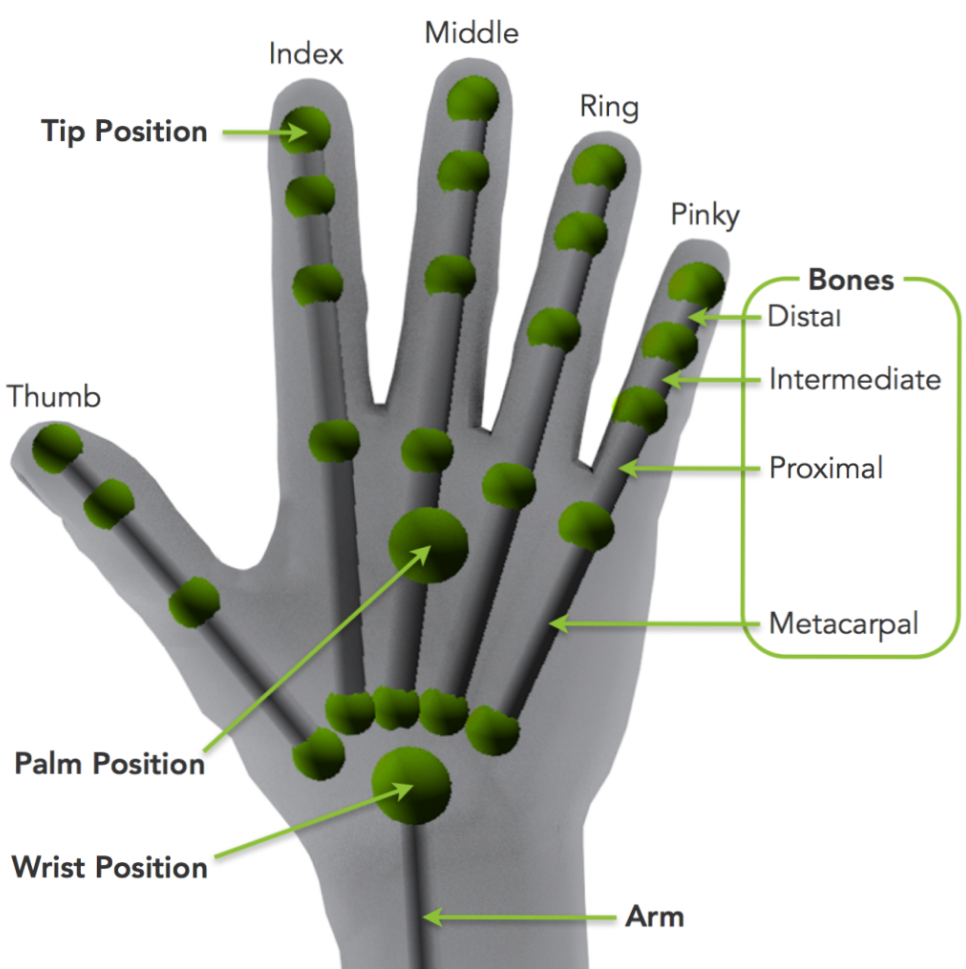
\includegraphics[scale=0.5]{Figures/handBones.png}
\caption[Hand Bone Model]{The Bones of the hand that Leap Motion device records data on. }
\label{fig:HandBones}
\end{figure}

A Hand object is only valid if it is detected by the Leap Motion device to be a physical object; if a Hand object is created via code using the Hand() constructor, that hand is considered “invalid” and will return true when the hand.invalid() method is called it. The information contained within a valid Hand object read in from the device is Read Only and can not be changed or updated. 

The Leap Motion device records numerical data about the hand and finger positions. Using the Hand class provided by the Leap Motion Java API and described above in the previous paragraph, a graphical model was constructed. For this GUI construction, a graphical representation of the hand was built using basic 3D geometric classes provided by the JavaFX framework. The bones of the hand model were represented by the Cylinder class and the joints were represented by the Sphere JavaFX class. This Hand model is contained inside the \verb UIHand_Simple Java class. This class extends a base abstract UIHand class which itself inherits from the JavaFX class called Group. Group is a type of Node in JavaFX that contains an ObservableList of children Nodes that will be added to the JavaFX Scene Graph in the order that they are added to the Group. An important point to note is that any transform, effect or property change applied to a Group will also be applied to all the children of that group. The Figure \ref{fig:javafxGroupNode} shows an example of how a Group Node can can contain multiple children nodes.

\begin{figure}[th]
\centering
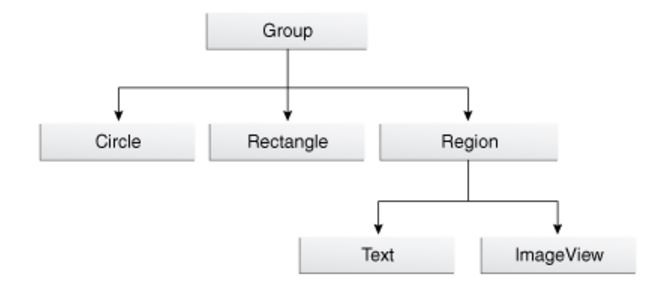
\includegraphics[scale=0.75]{Figures/javafx_group_node.JPG}
\caption[JavaFx Group Node]{The Group Node structure in the JavaFX framework. }
\label{fig:javafxGroupNode}
\end{figure}


The \verb UIHand_Simple class stores all the fingers bones in two dimensional array of Cylinder objects and all the respective joints in a different two dimensional array of Spheres. These arrays are of dimensions 5x3 to account for the five fingers and the three types of primary finger bones: distal, intermediate and proximal. In addition to these arrays, there is an array containing the four metacarpal bones of the hand; the thumb does not have a corresponding metacarpal bone like the other fingers. The also contains two more cylinders and a sphere to construct the palm section of the hand. To provide the hand with a uniform, well-blended color shading a PhongMaterial object is set as the hand’s material property. Figure \ref{fig:uihandsimpleConst} shows the initialization of the \verb UIHand_Simple and part of its constructor to illustrate how the hand model was designed.


\begin{figure}[th]
\centering
\begin{lstlisting}
public class UIHand_Simple extends UIHand {
    private static float fingerRadius = 14f;
	//Hand elements
    private Cylinder[][] fingerBones;
    private Sphere[][] fingerJoints;
    private Cylinder[] knuckleSpans;
	...
    public UIHand_Simple(Color color, boolean wireframe) {
        //Execute the Group constructor
        super();
        //Create the materials
        PhongMaterial dark = new PhongMaterial(color);
        PhongMaterial light = new PhongMaterial(color.brighter());
        //Initialize Finger bones
        fingerBones = new Cylinder[5][];
        for (int i = 0; i < 5; ++i) {
            fingerBones[i] = new Cylinder[3];
            for (int j = 0; j < 3; ++j) {
                fingerBones[i][j] = new Cylinder();
                //set material and radius and drawMode
                fingerBones[i][j].setMaterial(dark);
                fingerBones[i][j].setRadius(fingerRadius / ViewMath.radiusScaleFactor);
                if (wireframe) fingerBones[i][j].setDrawMode(DrawMode.LINE);
            }
		...
\end{lstlisting}
\caption[UIHandSimple Constructor]{A snippet of code showing how a the UIHandSimple class, representing the graphical hand, is constructed.}
\label{fig:uihandsimpleConst}
\end{figure}

Each element of the hand, such as all the cylinders and spheres representing the various bones and joints, is added to the children of the encompassing parent group that represents the hand.


%------------------------------------------------
%	SECTION 2 Set Location Method
%------------------------------------------------
\section{Set Location Method}
The \verb UIHand_Simple class also contains a method that allows for the graphical hand to be positioned according to the exact positions recorded in a Leap Motion Hand object. This method, which is called setLoc(Hand h), goes through each of the fingers and their respective bones and joints and sets the position and rotation of these these JavaFX nodes based upon the Hand object passed in. This method relies on a helper class called ViewMath which contains static methods that are called to position each individual cylinder representing a bone. Two of the important methods in ViewMath are setPositionByVector(Node n, Vector v) and setRotationByVector(Node n, Vector v). The method setPositionByVector sets the translate properties of the JavaFX Node passed in to the XYZ position recorded in the vector. The setRotationByVector method rotates the JavaFX Node passed into it by the direction which is represented by the second argument vector. This method first takes the direction and “corrects” it by flipping the z-value. This is done because JavaFX's coordinate system has the Z-axis increasing outward from the computer screen, while Leap Motion has the Z-axis increasing into the screen. The setRotationByVector finds the angle of rotation finding the the angle of the passed in direction to the Y-axis. In addition to the angle of rotation, the axis upon which the rotation will occur also needs to be defined. The axis of the rotation is found by taking the cross-product between the Y-axis and the “corrected” direction. Figure \ref{fig:setRotationByVectorCode} shows how rotation is set for nodes in the hand model.


\begin{figure}[th]
\centering
\begin{lstlisting}
//This method rotates a given JavaFx node to point in the direction passed in
public static void setRotationByVector(Node node, Vector direction) {
	//Correct the direction to correspond to JavaFx Coordinate system
	Vector correctedDirection = new Vector(direction.getX(), direction.getY(), -direction.getZ());
	//Find the angle of the direction to the y-axis; in degrees
	double angle = correctedDirection.angleTo(Vector.yAxis()) * 180 / Math.PI;
	//Find the axis of rotation by taking the cross product of the corrected direction with the y-axix
	Point3D axis = vectorToPoint(correctedDirection.cross(Vector.yAxis()));
	//Set the axis and angle of rotation on the Node object
	node.setRotate(angle);
	node.setRotationAxis(axis);
}
\end{lstlisting}
\caption[setRotationByVector Method]{A snippet of code showing how the rotation is set for an arbitrary Node object of the JavaFX Hand Model.}
\label{fig:setRotationByVectorCode}
\end{figure}




%------------------------------------------------
%	SECTION 3 Concurrency
%------------------------------------------------
\section{Concurrency}
One of the key concepts that is used in writing this project's application was that of concurrency. Concurrency in a JavaFX application is very important as it allows for the UI of to be responsive to user interactions despite the fact that the application might also be executing other tasks in the background. In other to achieve this requirement, it is necessary to employ multi-threading so that the main application thread can focus on responding to user interactions and other time-consuming tasks can be delegated to background threads. The UI in a JavaFX application is represented by the Scene Graph, which has been discussed earlier. The Scene Graph is not thread-safe and it should only be accessed and updated via the main running application thread, which is called the JavaFX Application thread. Implementing long running tasks on the JavaFX Application thread will invariably make the UI of the application unresponsive. The best practice is to avoid this problem by letting the JavaFX Application thread focus on just processing user events. 


%----------------------------------- JavaFX Concurrent Package
\subsection{JavaFX Concurrent Package}
%
One might consider implementing the Runnable interface and creating their own thread objects from scratch to employ in the multi-threaded environment required for building JavaFX applications. However, such an approach is not recommended; it can lead to unnecessary complexity and hard to debug problems such as deadlock, which is when competing threads are stuck waiting forever, and race conditions where critical data can be modified relatively simultaneously by two competing threads. Instead, it is much better to use the javafx.concurrent package and the classes contained within it to achieve the multi-threading required for a responsive application. The APIs provided by this package encode the best concurrent design implementations which allow for easy interaction with the UI and also ensure that such interactions happen on the appropriate thread of the program. 

To somebody who is familiar with Java technologies, he/she will know that Java already provides a complete set of concurrency related libraries in the java.util.concurrent package. However, these APIs are designed for traditional Java Abstract Data Types (ADTs) such as Lists, Maps etc. JavaFX applications usually are dealing with observable ADTs such as ObservableList and ObservableMap. The main difference between the observable ADTs and the traditional ADTs is that the observable ADTs allow for automatic synchronization between themselves and the view components of the UI. In web development lingo this is sometimes referred to as "two-way" data binding. It means means that if the data in the view changes changes, this change is automatically propagated to the underlying data structure without requiring any work on the programmer's part. Likewise if the observable model is updated with new data the view components will be updated to reflect that change as well. Because of this convenience observable ADTs are very much suited for use in building JavaFX applications. The javafx.concurrent package uses the existing APIs found in java.util.concurrent package and repurposes them to also take into account the observable ADTs. It also considers other constraints faced by GUI application developers such as the JavaFX Application thread and its primary role in handling UI interaction. 

Broadly speaking, the javafx.concurrent package consists of a Worker interface, which provides the APIs for communication between the background worker to the UI thread, and two classes called Task and Service, both of which implement the Worker Interface. Task is a fully observable implementation of the corresponding java.util.concurrent.FutureTask class. Therefore, this task class is very much suited for implementing asynchronous tasks in JavaFX that can handle user interaction and respond to events executed on the UI. This ability to handle user events is further displayed by the fact that the task class implements the EventTarget interface.  

%----------------------------------- Project Application
\subsection{Project Application}
%
Creating a custom task requires extending the Task class and implementing the call() method. The call() method is should contain code that only changes states which are safe to be modified from the background thread. Therefore the call() method cannot change the active scene graph nodes displayed on the screen as that may cause runtime exceptions. Nevertheless, since Task is designed to be used in GUI applications, it does have the ability to update observable data properties, change notifications for errors and cancellation of tasks, and respond to event being fired. Figure \ref{fig:staticEndTask} gives an example of one of the instances from the project which used a Task class to perform some work in the background thread as the UI was being refreshed to the main screen again. 

\begin{figure}[th]
\centering
\begin{lstlisting}
private static class StaticEndTask extends Task<Void> {
	@Override
	protected Void call() throws Exception {
		targetHand.setVisible(false);
		scene2Button.setVisible(true);
		...
	}
}
\end{lstlisting}
\caption[Task Class Code]{This shows part of the implementation of the Task class with call() method defined.}
\label{fig:staticEndTask}
\end{figure}

It is important to note that the Task class, since it implements the java.utils.concurrent.FutureTask class, fits into the traditional Java concurrency model also. The FutureTask class implements the Runnable interface, one of the key requirements for being able to be executed as a thread. Therefore, the Tasks can also can be used within the Java concurrency Executor API and also can be passed to a thread as a parameter. To see this fact in action, consider the Figure \ref{fig:platformRunLater} which shows a method that gets called when the user presses a button to go back to the main screen of the application. This snippet of code shows the Platform.runLater() method being passed various Tasks as parameters. The Platform.runLater() method can be called from any background thread and will add the passed tasks to a queue to be executed in order at a later time on the JavaFX Application thread and then this method returns immediately to the caller. Because of the concurrent behavior of the application, some of the methods in the application that deal with setting parameters and changing object data were initialized with the keyword "synchronized" which prevents multiple threads interferring with the same variables at the same time and generally preventing data consistency errors. 

\begin{figure}[th]
\centering
\begin{lstlisting}
public static void endStaticTest(double finalscore, long finaltime, boolean success) {
	Platform.runLater(new StaticScoreTask(finalscore, finaltime, success));
	try {
		Thread.sleep(5000);
	} catch (InterruptedException e) {
		// TODO Auto-generated catch block
		e.printStackTrace();
	}
	Platform.runLater(new StaticEndTask());
}
\end{lstlisting}
\caption[Passing Task as Parameter]{This code sample from the project shows Task objects being passed successfully to a method which expects to receive Runnable objects.}
\label{fig:platformRunLater}
\end{figure}

